\documentclass[14pt]{extreport}
\usepackage{cmap}
\usepackage[utf8]{inputenc}
\usepackage[english,ukrainian]{babel}
\usepackage{graphicx}
\usepackage{geometry}
\usepackage{listings}
\usepackage{amsmath}
\usepackage{float}
\geometry{
	a4paper,
	left=20mm,
	right=20mm,
	top=20mm,
	bottom=20mm
}
\lstset{
	language=bash,
	tabsize=4,
	breaklines,
	keepspaces,
	showstringspaces=false,
}
\graphicspath{ {./pictures} }
\setlength{\parindent}{4em}

\newcommand\subject{Бази даних}
\newcommand\lecturer{асистент кафедри ПЗ\\Білоіваненко М.В.}
\newcommand\teacher{асистент кафедри ПЗ\\Майхер В.Ю.}
\newcommand\mygroup{ПЗ-32}
\newcommand\lab{2}
\newcommand\theme{Cтворення бази даних засобами графічного інтерфейсу програми PgAdmin}
\newcommand\purpose{творення бази даних засобами графічного інтерфейсу програми PgAdmin: створення таблиць, створення зв’язків між таблицями.}

\begin{document}
\begin{normalsize}
	\begin{titlepage}
		\thispagestyle{empty}
		\begin{center}
			\textbf{МІНІСТЕРСТВО ОСВІТИ І НАУКИ УКРАЇНИ\\
				НАЦІОНАЛЬНИЙ УНІВЕРСИТЕТ "ЛЬВІВСЬКА ПОЛІТЕХНІКА"}
		\end{center}
		\begin{flushright}
			Інститут \textbf{КНІТ}\\
			Кафедра \textbf{ПЗ}
		\end{flushright}
		\vspace{200pt}
		\begin{center}
			\textbf{ЗВІТ}\\
			\vspace{10pt}
			До лабораторної роботи № \lab\\
			\textbf{На тему}: “\textit{\theme}”\\
			\textbf{З дисципліни}: “\subject”
		\end{center}
		\vspace{40pt}
		\begin{flushright}
			
			\textbf{Лектор}:\\
			\lecturer\\
			\vspace{10pt}
			\textbf{Виконав}:\\
			
			студент групи \mygroup\\
			Коваленко Д.М.\\
			\vspace{10pt}
			\textbf{Прийняв}:\\
			
			\teacher\\
			
			\vspace{28pt}
			«\rule{1cm}{0.15mm}» \rule{1.5cm}{0.15mm} 2023 р.\\
			$\sum$ = \rule{1cm}{0.15mm}……………\\
			
		\end{flushright}
		\vspace{\fill}
		\begin{center}
			\textbf{Львів — 2023}
		\end{center}
	\end{titlepage}
		
	\begin{description}
		\item[Тема.] \theme.
		\item[Мета.] \purpose.
	\end{description}

	\section*{Лабораторне завдання}
	\begin{enumerate}
		\item В СУБД PostgreSQL створити навчальну базу даних "Операції купівлі-продажу". Назва бази даних повинна містити прізвище власника.
		\item В СУБД PostreSQL за допомогою графічного інтерфейсу створити таблиці бази даних "Операції купівлі-продажу" та базу даних індивідуального завдання.
		\item В СУБД PostgreSQL за допомогою графічного інтерфейсу побудувати діаграму бази даних "Операції купівлі-продажу" та базу даних індивідуального завдання.
		\item Оформити звіт.
	\end{enumerate}
	
	\section*{Хід роботи}
	\subsection*{База даних "Операції купівлі-продажу"}
	
	\begin{figure}[H]
		\centering
		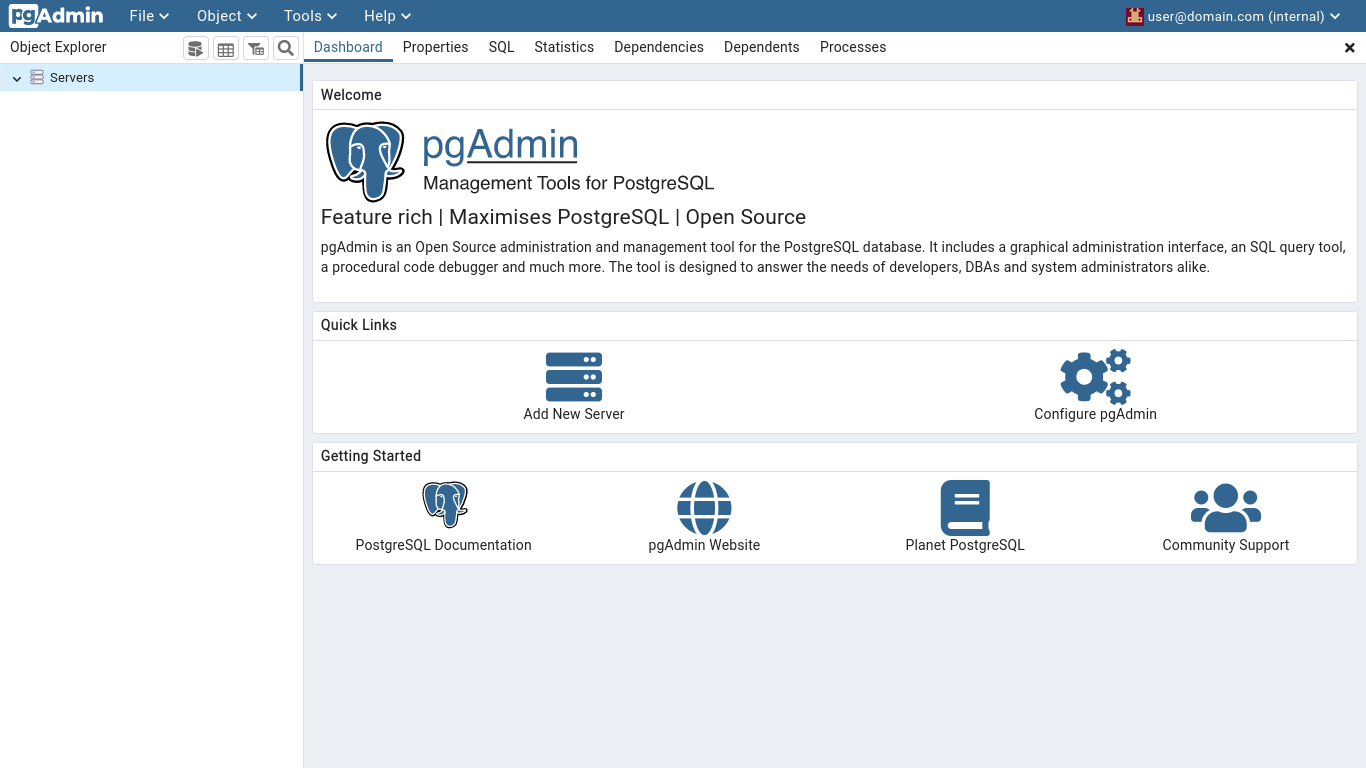
\includegraphics[scale=0.35]{1}
		\caption{Головна сторінка PgAdmin}
	\end{figure}

	\begin{figure}[H]
		\centering
		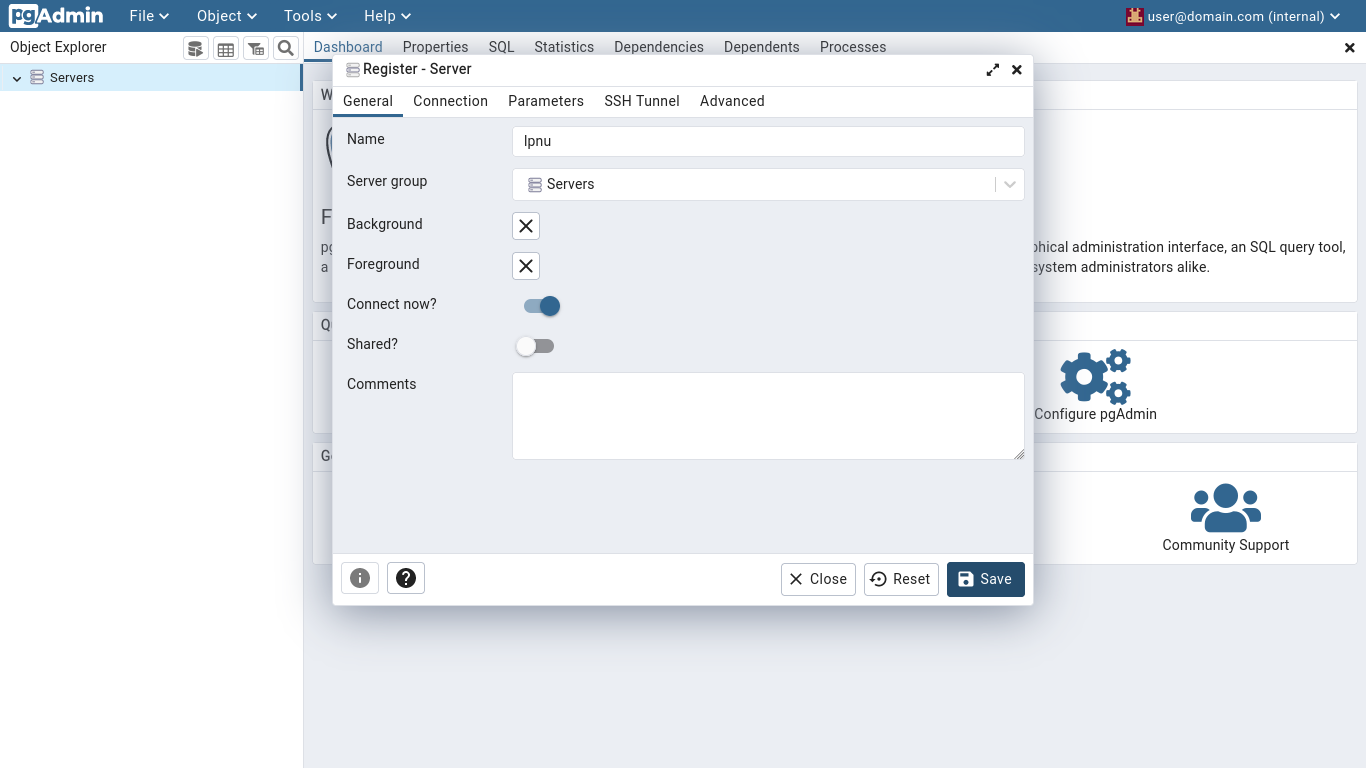
\includegraphics[scale=0.35]{2}
		\caption{Під'єднання до сервера PostgreSQL}
	\end{figure}
	
	\begin{figure}[H]
		\centering
		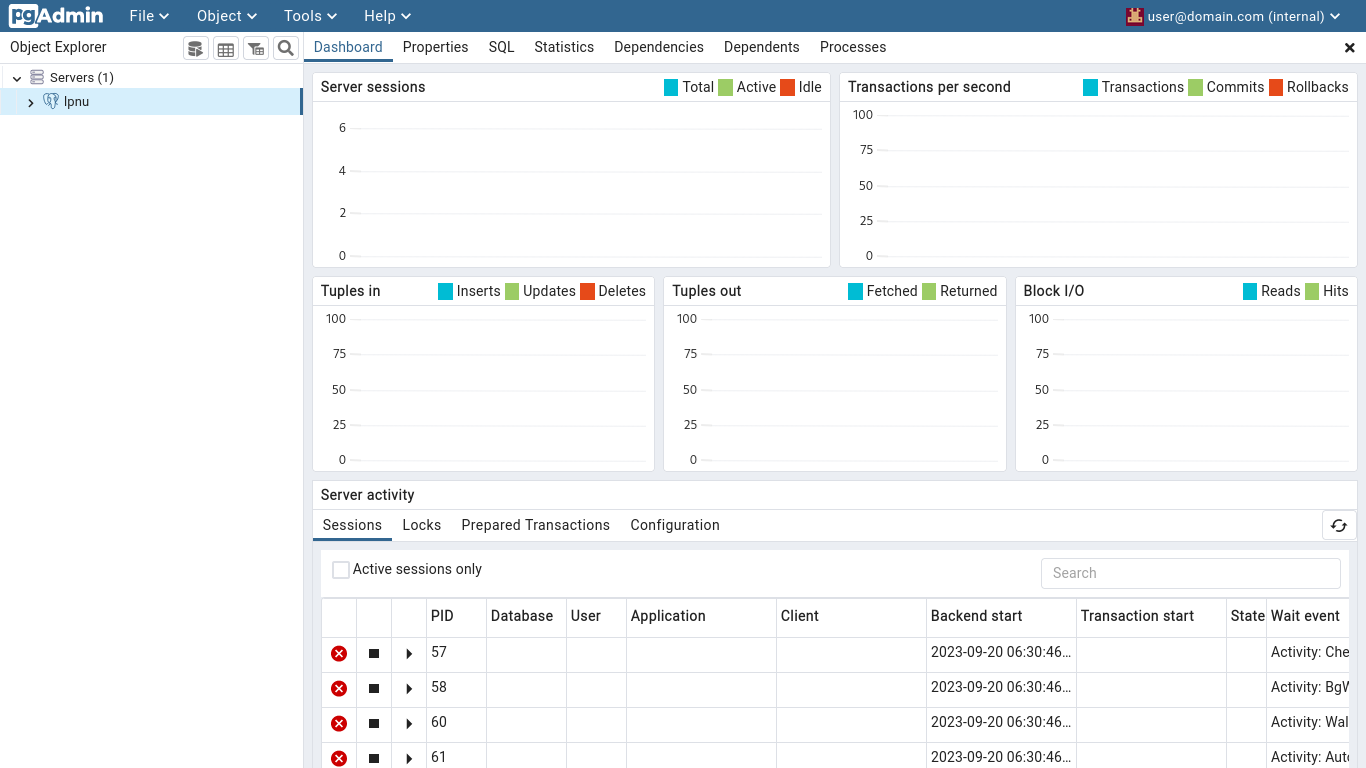
\includegraphics[scale=0.35]{3}
		\caption{Сторінка огляду сервера PostgreSQL}
	\end{figure}
	
	\begin{figure}[H]
		\centering
		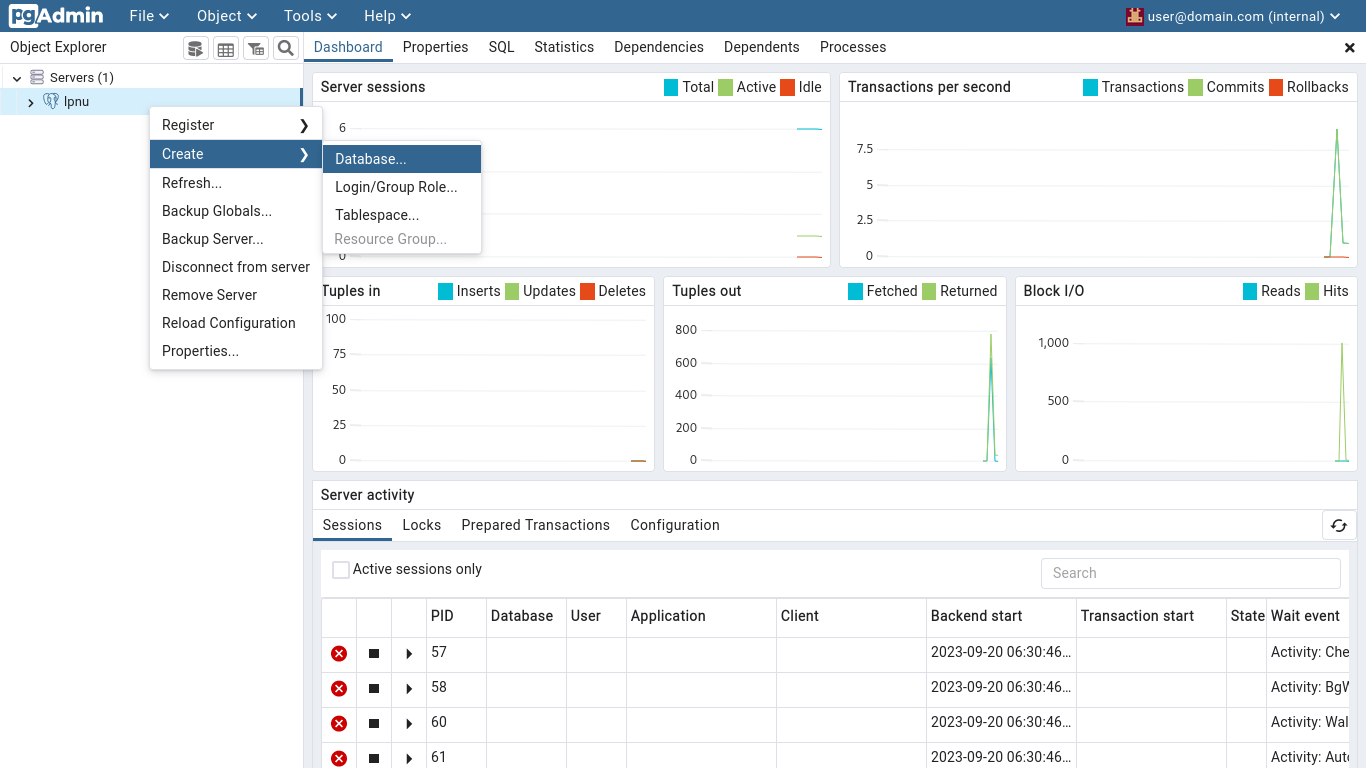
\includegraphics[scale=0.35]{4}
		\caption{Створення бази даних}
	\end{figure}
	
	\begin{figure}[H]
		\centering
		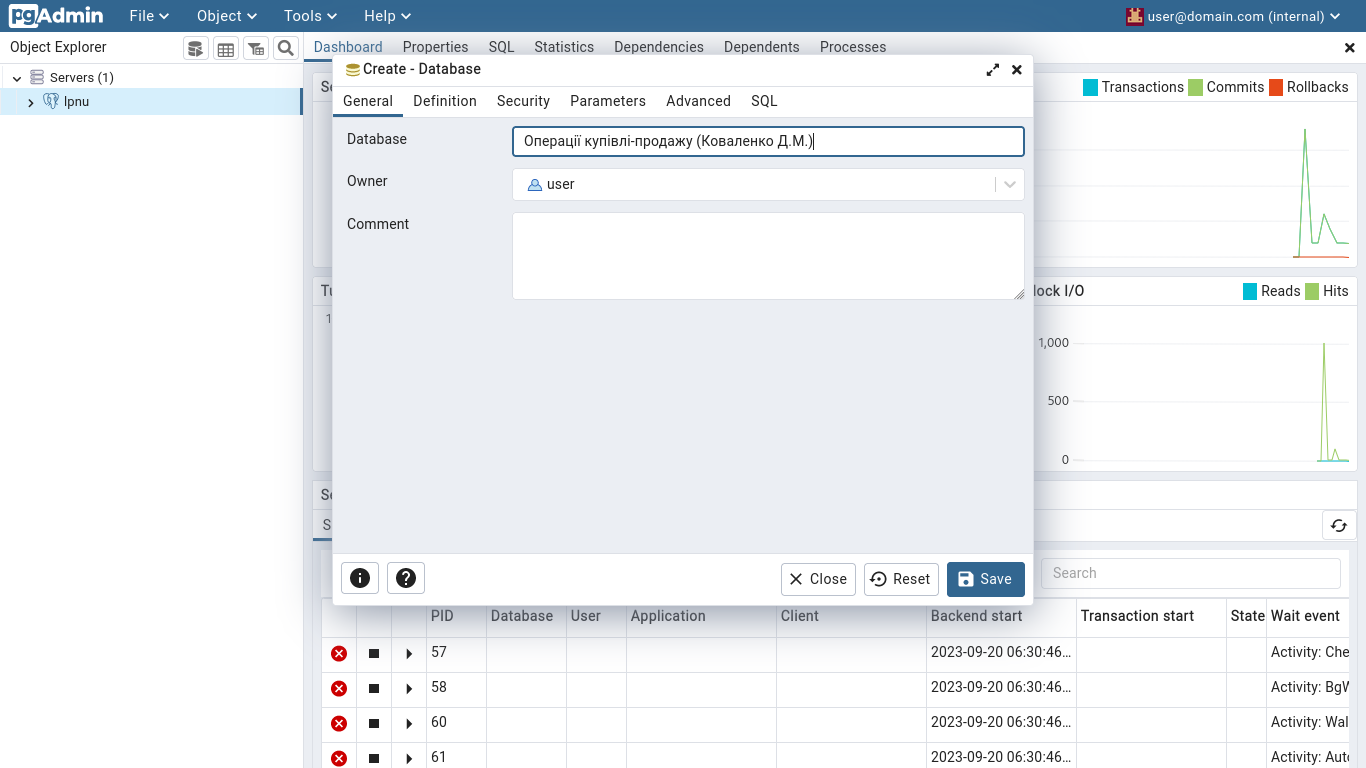
\includegraphics[scale=0.35]{5}
		\caption{Створення бази даних}
	\end{figure}
	
	\begin{figure}[H]
		\centering
		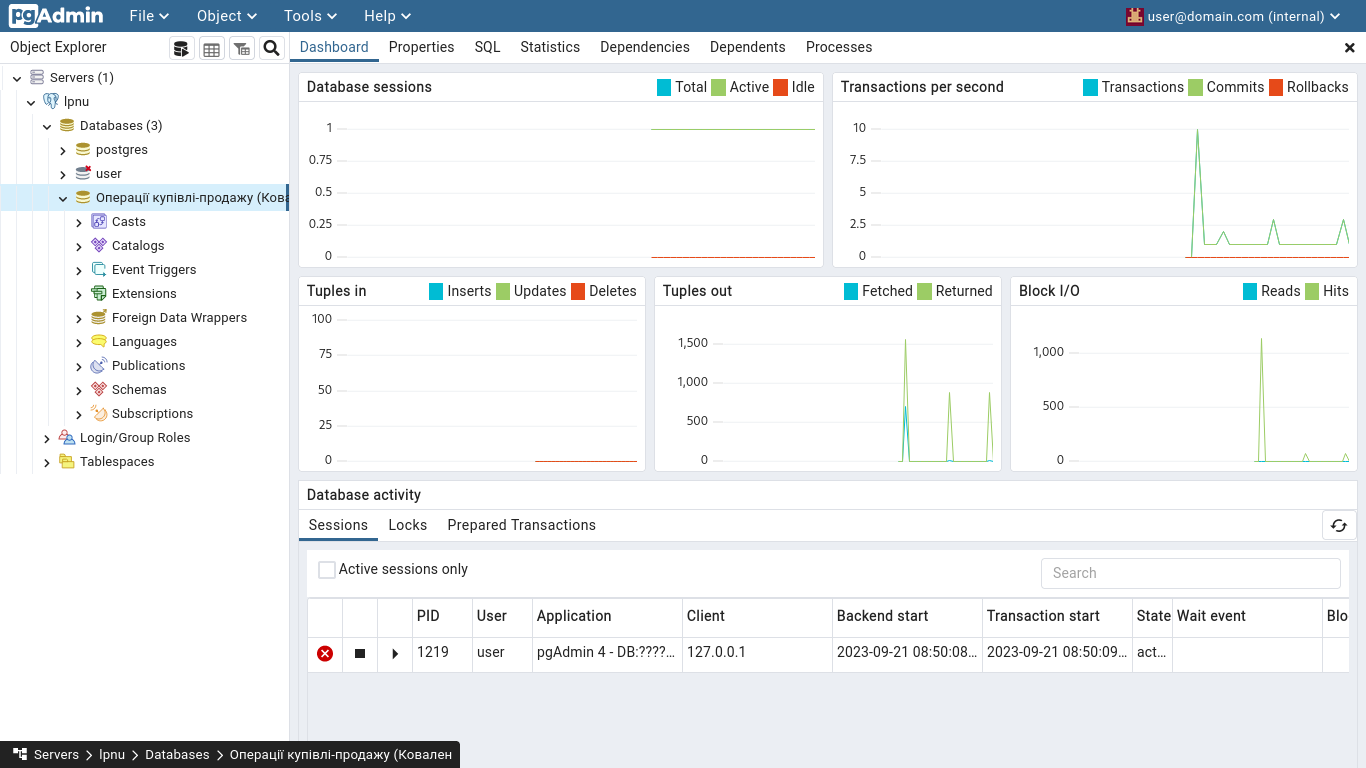
\includegraphics[scale=0.35]{7}
		\caption{Сторінка огляду бази даних}
	\end{figure}
	
	\begin{figure}[H]
		\centering
		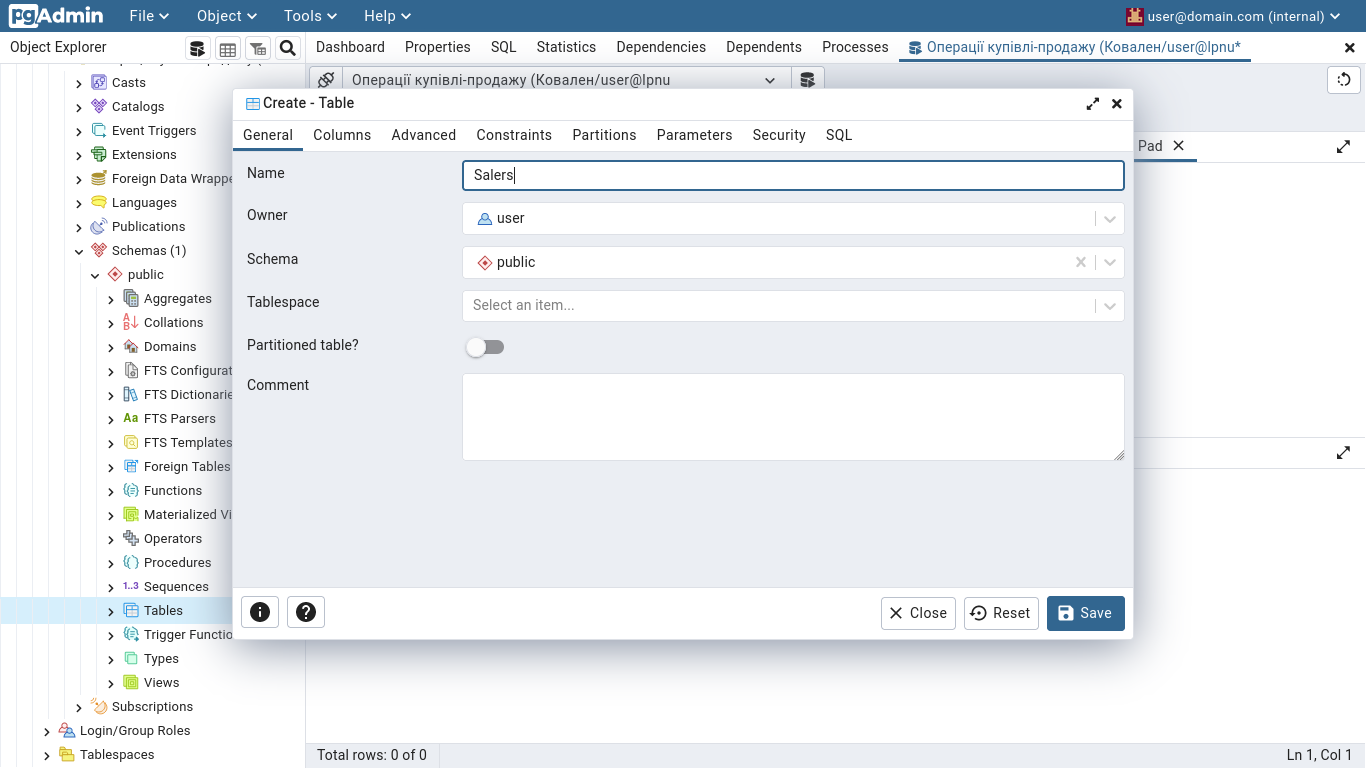
\includegraphics[scale=0.35]{8}
		\caption{Створення таблиці Salers}
	\end{figure}
	
	\begin{figure}[H]
		\centering
		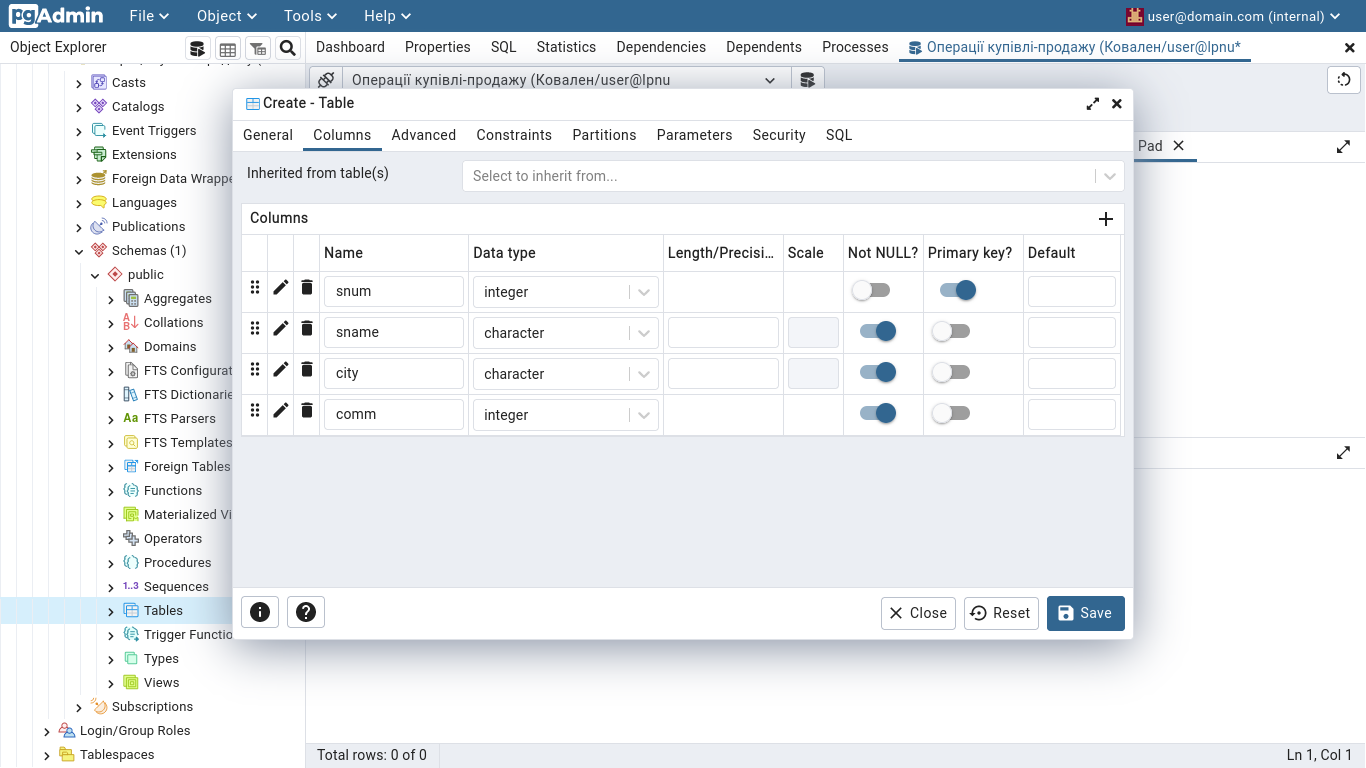
\includegraphics[scale=0.35]{9}
		\caption{Створення полів таблиці Salers}
	\end{figure}
	
	\begin{figure}[H]
		\centering
		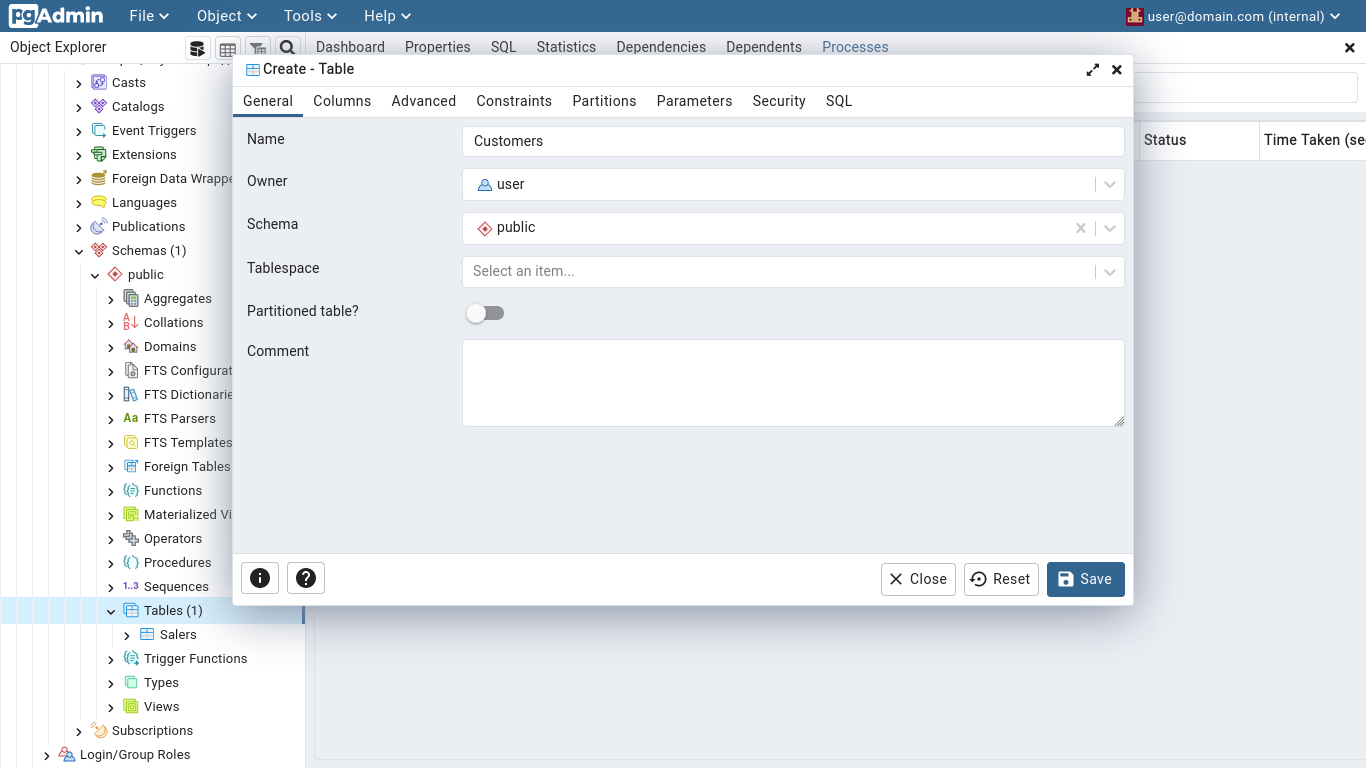
\includegraphics[scale=0.35]{10}
		\caption{Створення таблиці Customers}
	\end{figure}
	
	\begin{figure}[H]
		\centering
		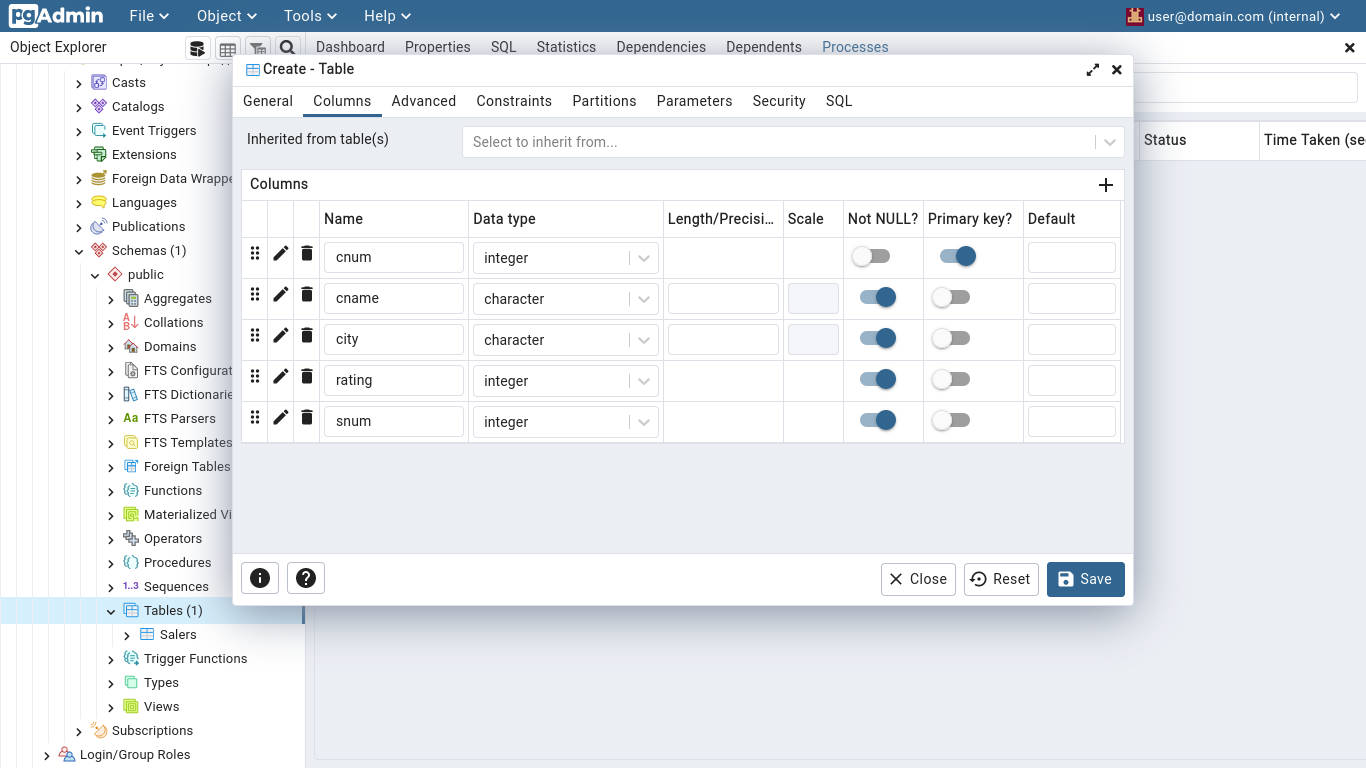
\includegraphics[scale=0.35]{11}
		\caption{Створення полів таблиці Customers}
	\end{figure}
	
	\begin{figure}[H]
		\centering
		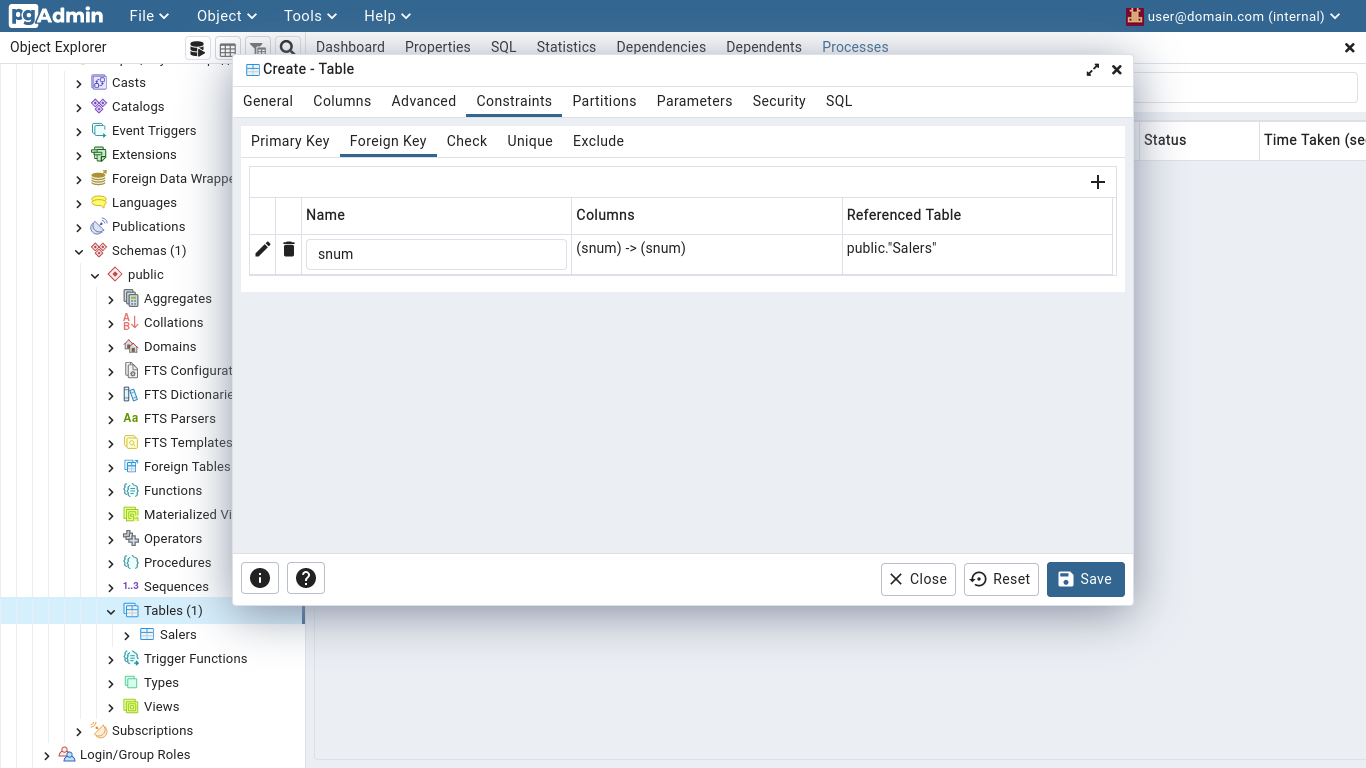
\includegraphics[scale=0.35]{12}
		\caption{Створення полів таблиці Customers}
	\end{figure}
	
	\begin{figure}[H]
		\centering
		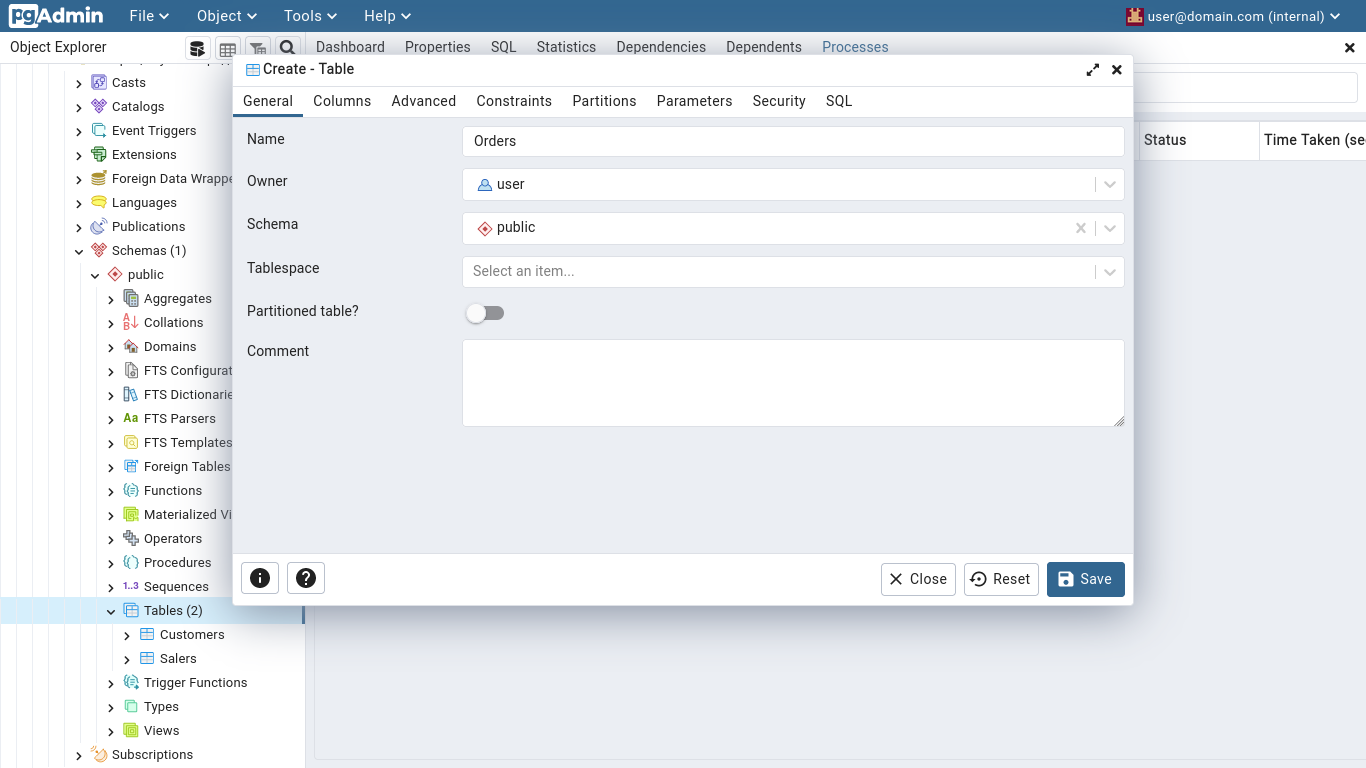
\includegraphics[scale=0.35]{13}
		\caption{Створення таблиці Orders}
	\end{figure}
	
	\begin{figure}[H]
		\centering
		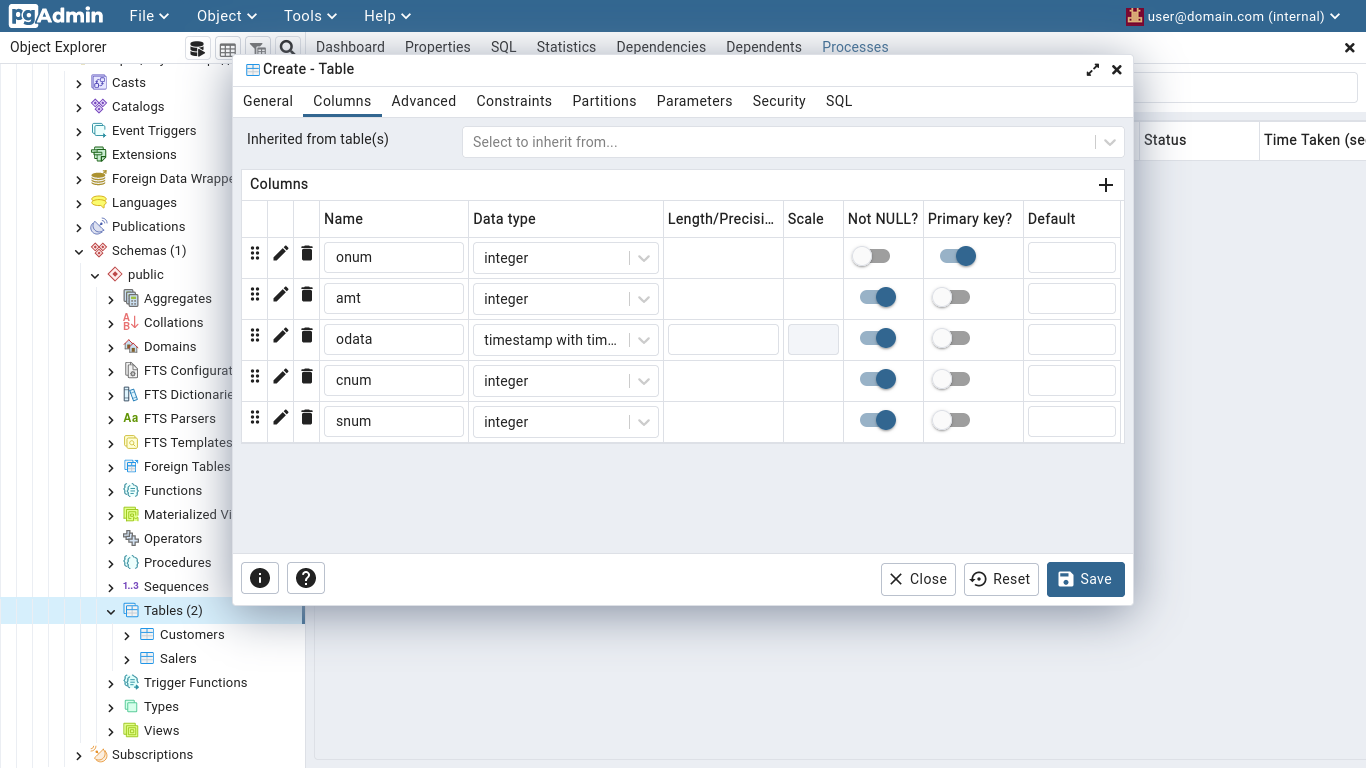
\includegraphics[scale=0.35]{14}
		\caption{Створення полів таблиці Orders}
	\end{figure}
	
	\begin{figure}[H]
		\centering
		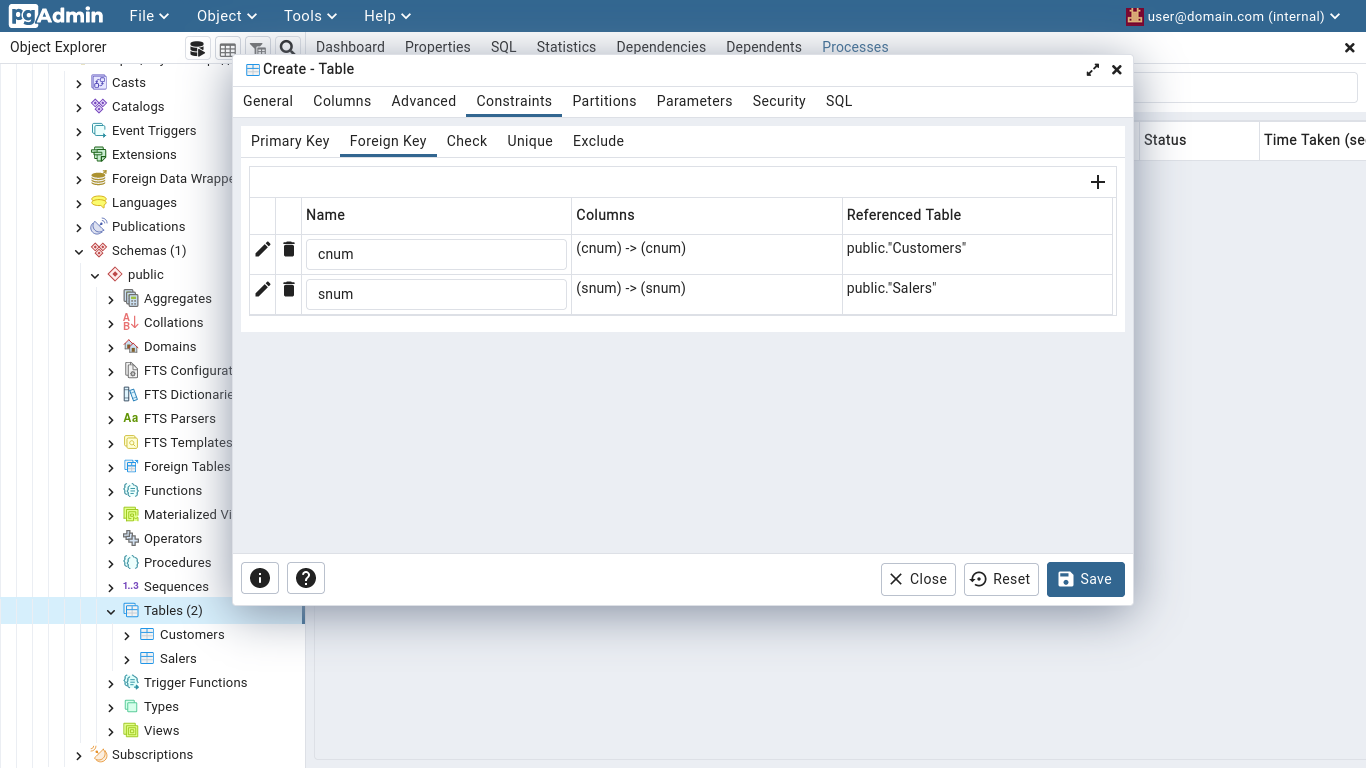
\includegraphics[scale=0.35]{15}
		\caption{Створення полів таблиці Orders}
	\end{figure}
	
	\begin{figure}[H]
		\centering
		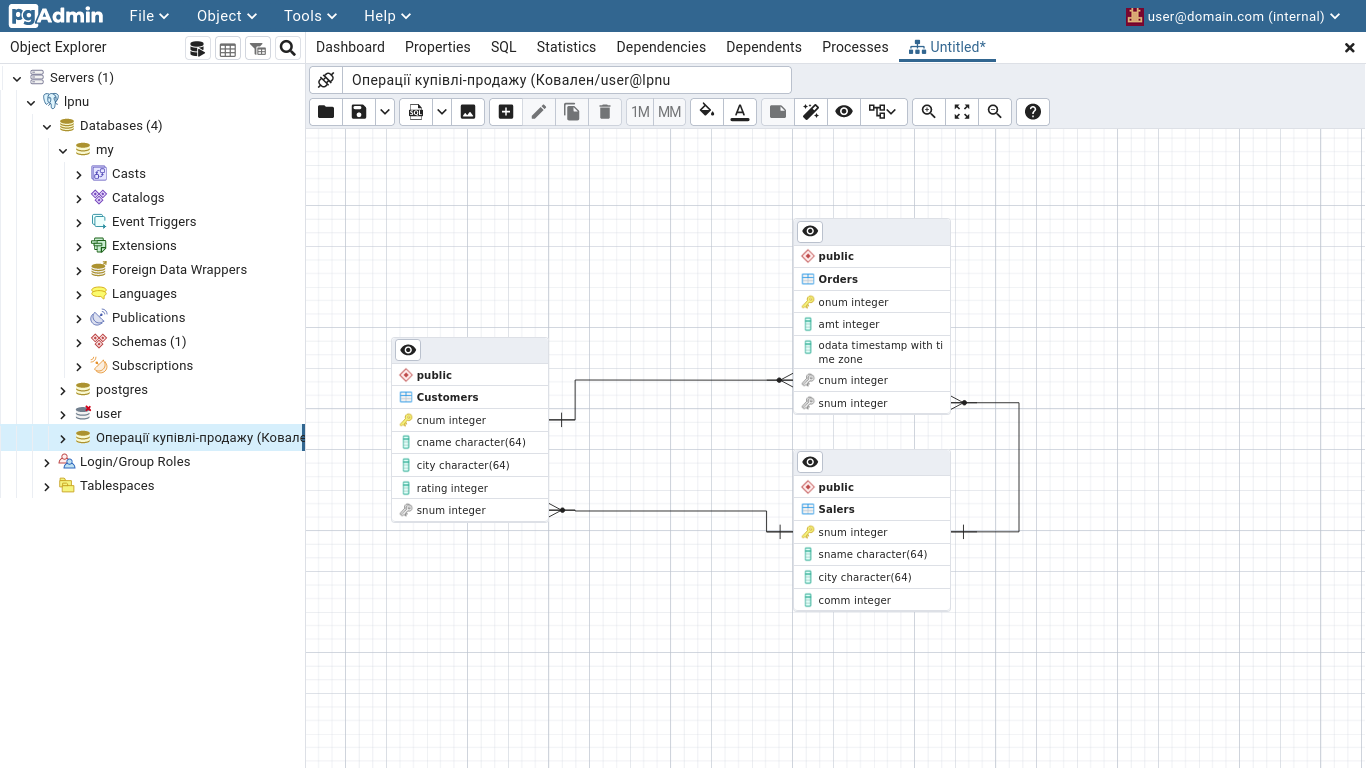
\includegraphics[scale=0.35]{16}
		\caption{Діаграма бази даних "Операції купівлі-продажу"}
	\end{figure}

	\subsection*{База даних індивідуального завдання}
	Варіант: база даних для роботи компанії з регулярних перевезень пасажирів.

	timetable:
	\begin{itemize}
		\item id
		\item route\_id
		\item vehicle\_id
		\item departure\_time
		\item arrival\_time
	\end{itemize}

	routes:
	\begin{itemize}
		\item id
		\item name
		\item distance
	\end{itemize}
	
	stops:
	\begin{itemize}
		\item id
		\item name
		\item coords
	\end{itemize}
	
	route\_stops:
	\begin{itemize}
		\item id
		\item route\_id
		\item stop\_id
		\item order\_index
	\end{itemize}

	vehicles:
	\begin{itemize}
		\item id
		\item type
		\item status
		\item route
		\item coords
		\item license\_plate
		\item capacity
	\end{itemize}

	passangers:
	\begin{itemize}
		\item id
		\item name
		\item email
		\item password
	\end{itemize}

	feedbacks:
	\begin{itemize}
		\item id
		\item passenger\_id
		\item time
		\item 
	\end{itemize}

	\section*{Висновок}
	Під час виконання лабораторної роботи я встановив та налаштував PostgreSQL та PgAdmin. Для виконання лабораторної роботи я обрав шлях для встановлення та налаштування необхідних програмних компонентів за допомогою контейнеризованого оточення. Я здобув необхідні навички для роботи з PostgreSQL та pgAdmin.
	 
\end{normalsize}
\end{document}
